\chapter{Tecnologías utilizadas}\label{chapter:Tecnologias_utilizadas}

El objetivo general de este proyecto se basa en construir un prototipo de robot humanoide que sea capaz de detectar la cercanía
de una pelota, acercarse a ella y patearla, reincorporandose a la posicion de pie en caso de perder el equilibrio y caer
mientras camina. Para cumplir con este objetivo se han desglosado un conjunto de objetivos específicos que se describen 
acontinuación: 

\begin{enumerate}
\item  Diseño y construcción de un humanoide con piezas del kit de robótica Bioloid Premium, sustituyendo su tarjeta controladora
CM-530 por la tarjeta de software libre ArbotiX para controlar los motores Dynamixel y otros sensores.
\begin{enumerate}
\item Instalación y configuración de la tarjeta ArbotiX.
\item Instalación y configuración de la tarjeta Raspberry Pi.
\item Instalación y configuración de la cámara Raspberry Pi.
\item Instalación de servomotores  para el movimiento de la cámara
\item Instalación del giroscopio Gyro.
 
\end{enumerate}
\end{enumerate}

\begin{enumerate}
\item Detección de la pelota
\begin{enumerate}
\item  Captura de imagen con la cámara Raspberry Pi a través de la librería raspicam cv.
\item Procesamiento de la imagen para extraer información de la posición de la pelota con las librerías de OpenCV.
\end{enumerate}

\end{enumerate}

\begin{enumerate}
\item Búsqueda de la pelota y pateo de la misma. 
\begin{enumerate}
\item Creación de las poses necesarias para caminar, girar, levantarse y patear usando el software pypose.
\item Programación de transiciones de movimientos.
\item Control de servomotores para el movimiento de la cámara.
\item Establecer mecanismo de comunicación entre la tarjetas ArbotiX y Raspberry Pi.  
\item Programación de algoritmo de planificación de acciones que lleve al humanoide a acercarse a la pelota.
\item Detección de movimientos angulares bruscos que sugieran una caída, a través de la lectura del giroscopio
\item Identificación del momento en que la pelota se encuentre en una zona adecuada para patear.
\end{enumerate}
\end{enumerate}

\section{ Herramientas de software}
En esta sección se describen las herramientas de software utilizadas para la programación del proyecto.
\begin{itemize}
\item Pypose: Software especializado en el control de los servomotores Dynamixel Ax-12. Una de las más importantes
características es que, luego de haber fijado a mano las posiciones de los motores, permite la lectura simultánea de esas
posiciones para captar la pose del robot. Con esta herramienta es posible formar una secuencia de poses que generen un
movimiento, por ejemplo, caminar. \cite{pypose}

\item ROS: ROS (Robot Operating System) es un framework que proporciona bibliotecas y herramientas para ayudar a los desarrolladores de software a crear aplicaciones robóticas. Proporciona abstracción de hardware, controladores de dispositivos, bibliotecas, visualizadores, paso de mensajes, gestión de paquetes y más. ROS se encuentra bajo licencia de código abierto, la licencia BSD.

\item OpenCv (Open Source Computer Vision Library): Es una librería de visión de computadoras y aprendizaje de máquinas de código abierto. Ha sido diseñada para acelerar el uso de la percepción de maquinas y para proveer una estructura común en las aplicaciones de visión de computadoras. Registrada bajo la licencia BSD, de código abierto. \cite{opencv}

\item IDE Arduino: Es un entorno de desarrollo para escribir y cargar código en la tarjeta Arduino. Otras tarjetas
con microcontroladores AVR también son compatibles, como la ArbotiX. El lenguaje de programación del IDE de Arduino es una
implementación de Wiring el cual esta basado en Processing.  \cite{arduino}

\end{itemize}


\section{Componentes de hardware}
En esta sección se describen los principales componentes utilizados para armar la estructura del robot.
\begin{itemize}
\item Bioloid Premium kit: Es un kit de robótica con piezas modulares que permite armar diferentes tipos de robot pero 
principalmente humanoides. El fabricante, ROBOTIS, incluye un manual con varios modelos de robots con instrucciones de 
ensamblaje. Provee una tarjeta controladora, CM-530, a la que se conectan los motores Dynamixel y algunos sensores que se 
programan a través de la interfaz de ‘RoboPlus’. \cite{robotics}

\end{itemize}

\begin{figure}[hbtp]

\centering
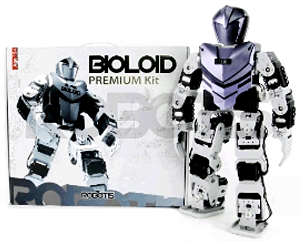
\includegraphics[scale=0.5]{imagenes/product_bioloid17.png}
\caption{Bioloid Premium Kit}
\end{figure}

\begin{itemize}

\item Motores Dynamixel Ax-12+: Son actuadores inteligentes y modulares que incorporan un reductor de engranajes, un motor DC
de presión y un circuito de control con funcionalidad de red, todo en un solo paquete \cite{manual}. 
\end{itemize}

\begin{figure}[hbtp]

\centering
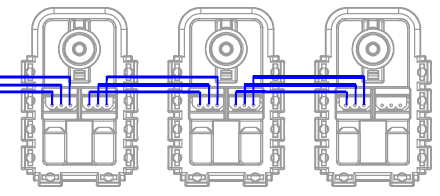
\includegraphics[scale=0.5]{imagenes/AX-12_serie.png}
\caption{Motores Dynamixel conectados en serie}
\end{figure}

\begin{itemize}
\item Gyro: Es un giroscopio de la marca Robotis que mide la velocidad angular, diseñado para mantener el balance del robot y
ser usado para otras aplicaciones de movimiento. \cite{gyro} 

\end{itemize}

\begin{figure}[hbtp]
\centering
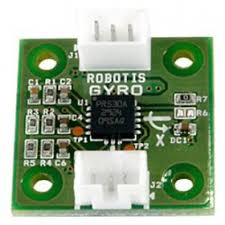
\includegraphics[scale=0.5]{imagenes/gyro.jpg}
\caption{Sensor Gyro}
\end{figure}

\begin{itemize}
\item Arbotix: El controlador ArbotiX es una solución de control avanzado para manejar servos Dynamixel AX/MX/RX/EX y robots
basados en Bioloid. Incorpora un potente microcontrolador AVR, radio inalámbrica XBEE, conductores de motor dual, y cabeceras
de estilo servo de 3 pines para E/S digital y analógica.\cite{arbotix}

\end{itemize}

%\begin{figure}[hbtp]
%\centering
%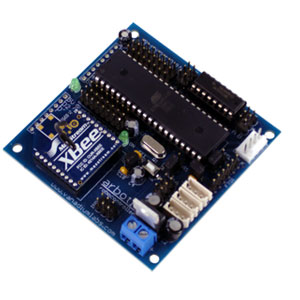
\includegraphics[scale=0.5]{imagenes/ARBOTIX.JPG}
%\caption{Tarjeta controladora ArbotiX}
%\end{figure}

\begin{itemize}
\item FTDI (Future Technology Devices International) : Es una tarjeta controladora que ofrece el servicio de conversión de 
datos de USB a UART. Permite la comunicación entre diferentes dispositivos \cite{ftdi}.

\end{itemize}

\begin{figure}[hbtp]
\centering
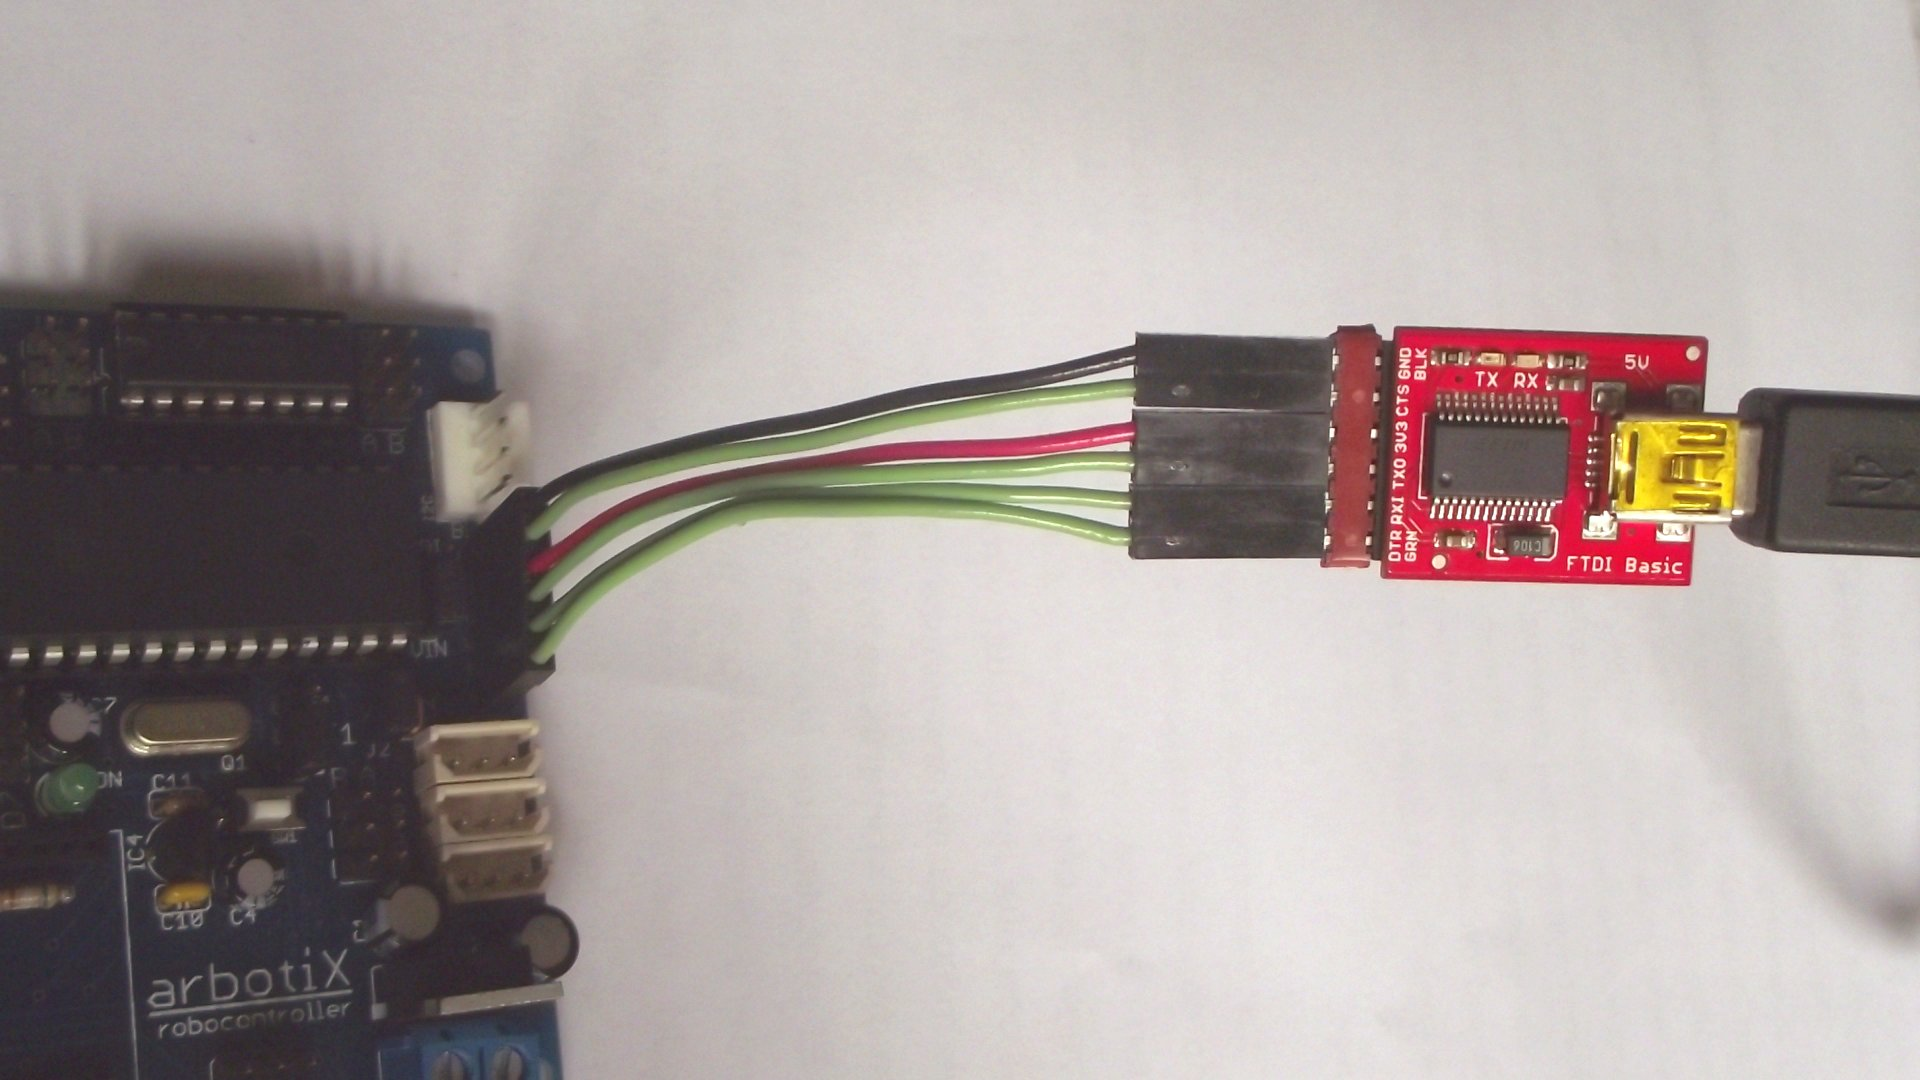
\includegraphics[scale=0.09]{imagenes/DSCF1162.jpg}
\caption{Chip FTDI conectado a la tarjeta Arbotix}
\end{figure}

\begin{itemize}
\item Extensor de puertos bioloid : Permite aumentar el número de cadenas de servos conectados a la tarjeta. \cite{hub} 
\end{itemize}

\begin{figure}[hbtp]
\centering
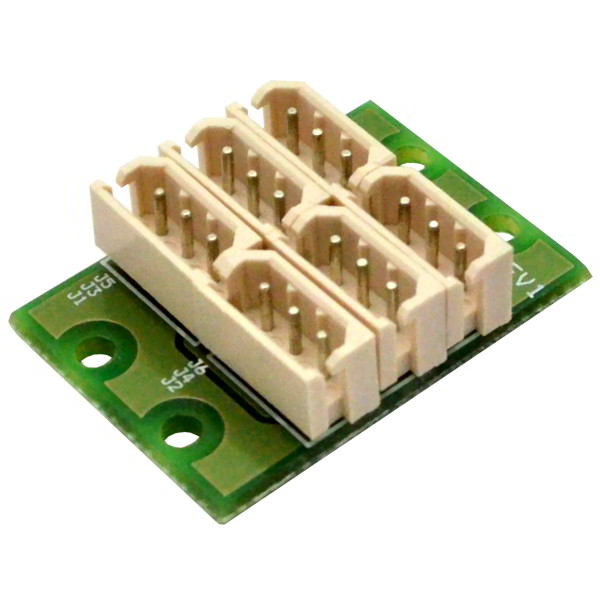
\includegraphics[scale=0.3]{imagenes/Dynamixel-AX-MX-6-Port-Extension-Hub-600x600.jpg}
\caption{Extensor de puertos bioloid}
\end{figure}

\begin{itemize}
\item Servo motor analogico micro TG9 e: Es un pequeño servomotor cuyo torque alcanza 1.50 kg-cm y una velocidad de 60 por
segundo. Permite ser controlado en posición en un rango de 180. \cite{microservo}  

\end{itemize}

\begin{figure}[hbtp]
\centering
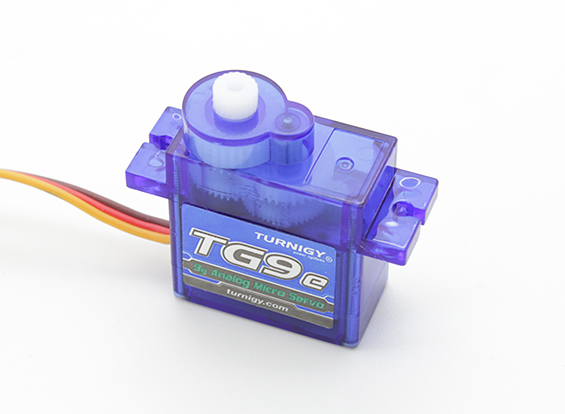
\includegraphics[scale=0.3]{imagenes/turnigy.jpg}
\caption{Servo motor analógico}
\end{figure}

\begin{itemize}
\item Raspberry Pi: La Raspberry Pi es un ordenador del tamaño de una tarjeta de crédito a la que se puede conectar un 
televisor y un teclado. Se trata de un pequeño ordenador capaz de ser utilizado en proyectos de electrónica, y para muchas 
de las tareas que una PC de escritorio hace, como hojas de cálculo, procesadores de texto y juegos \cite{raspberry}. 

\end{itemize}

%imagen tomada de: %http://rayhightower.com/blog/2012/12/03/ruby-on-raspberry-pi/
\begin{figure}[hbtp]
\centering
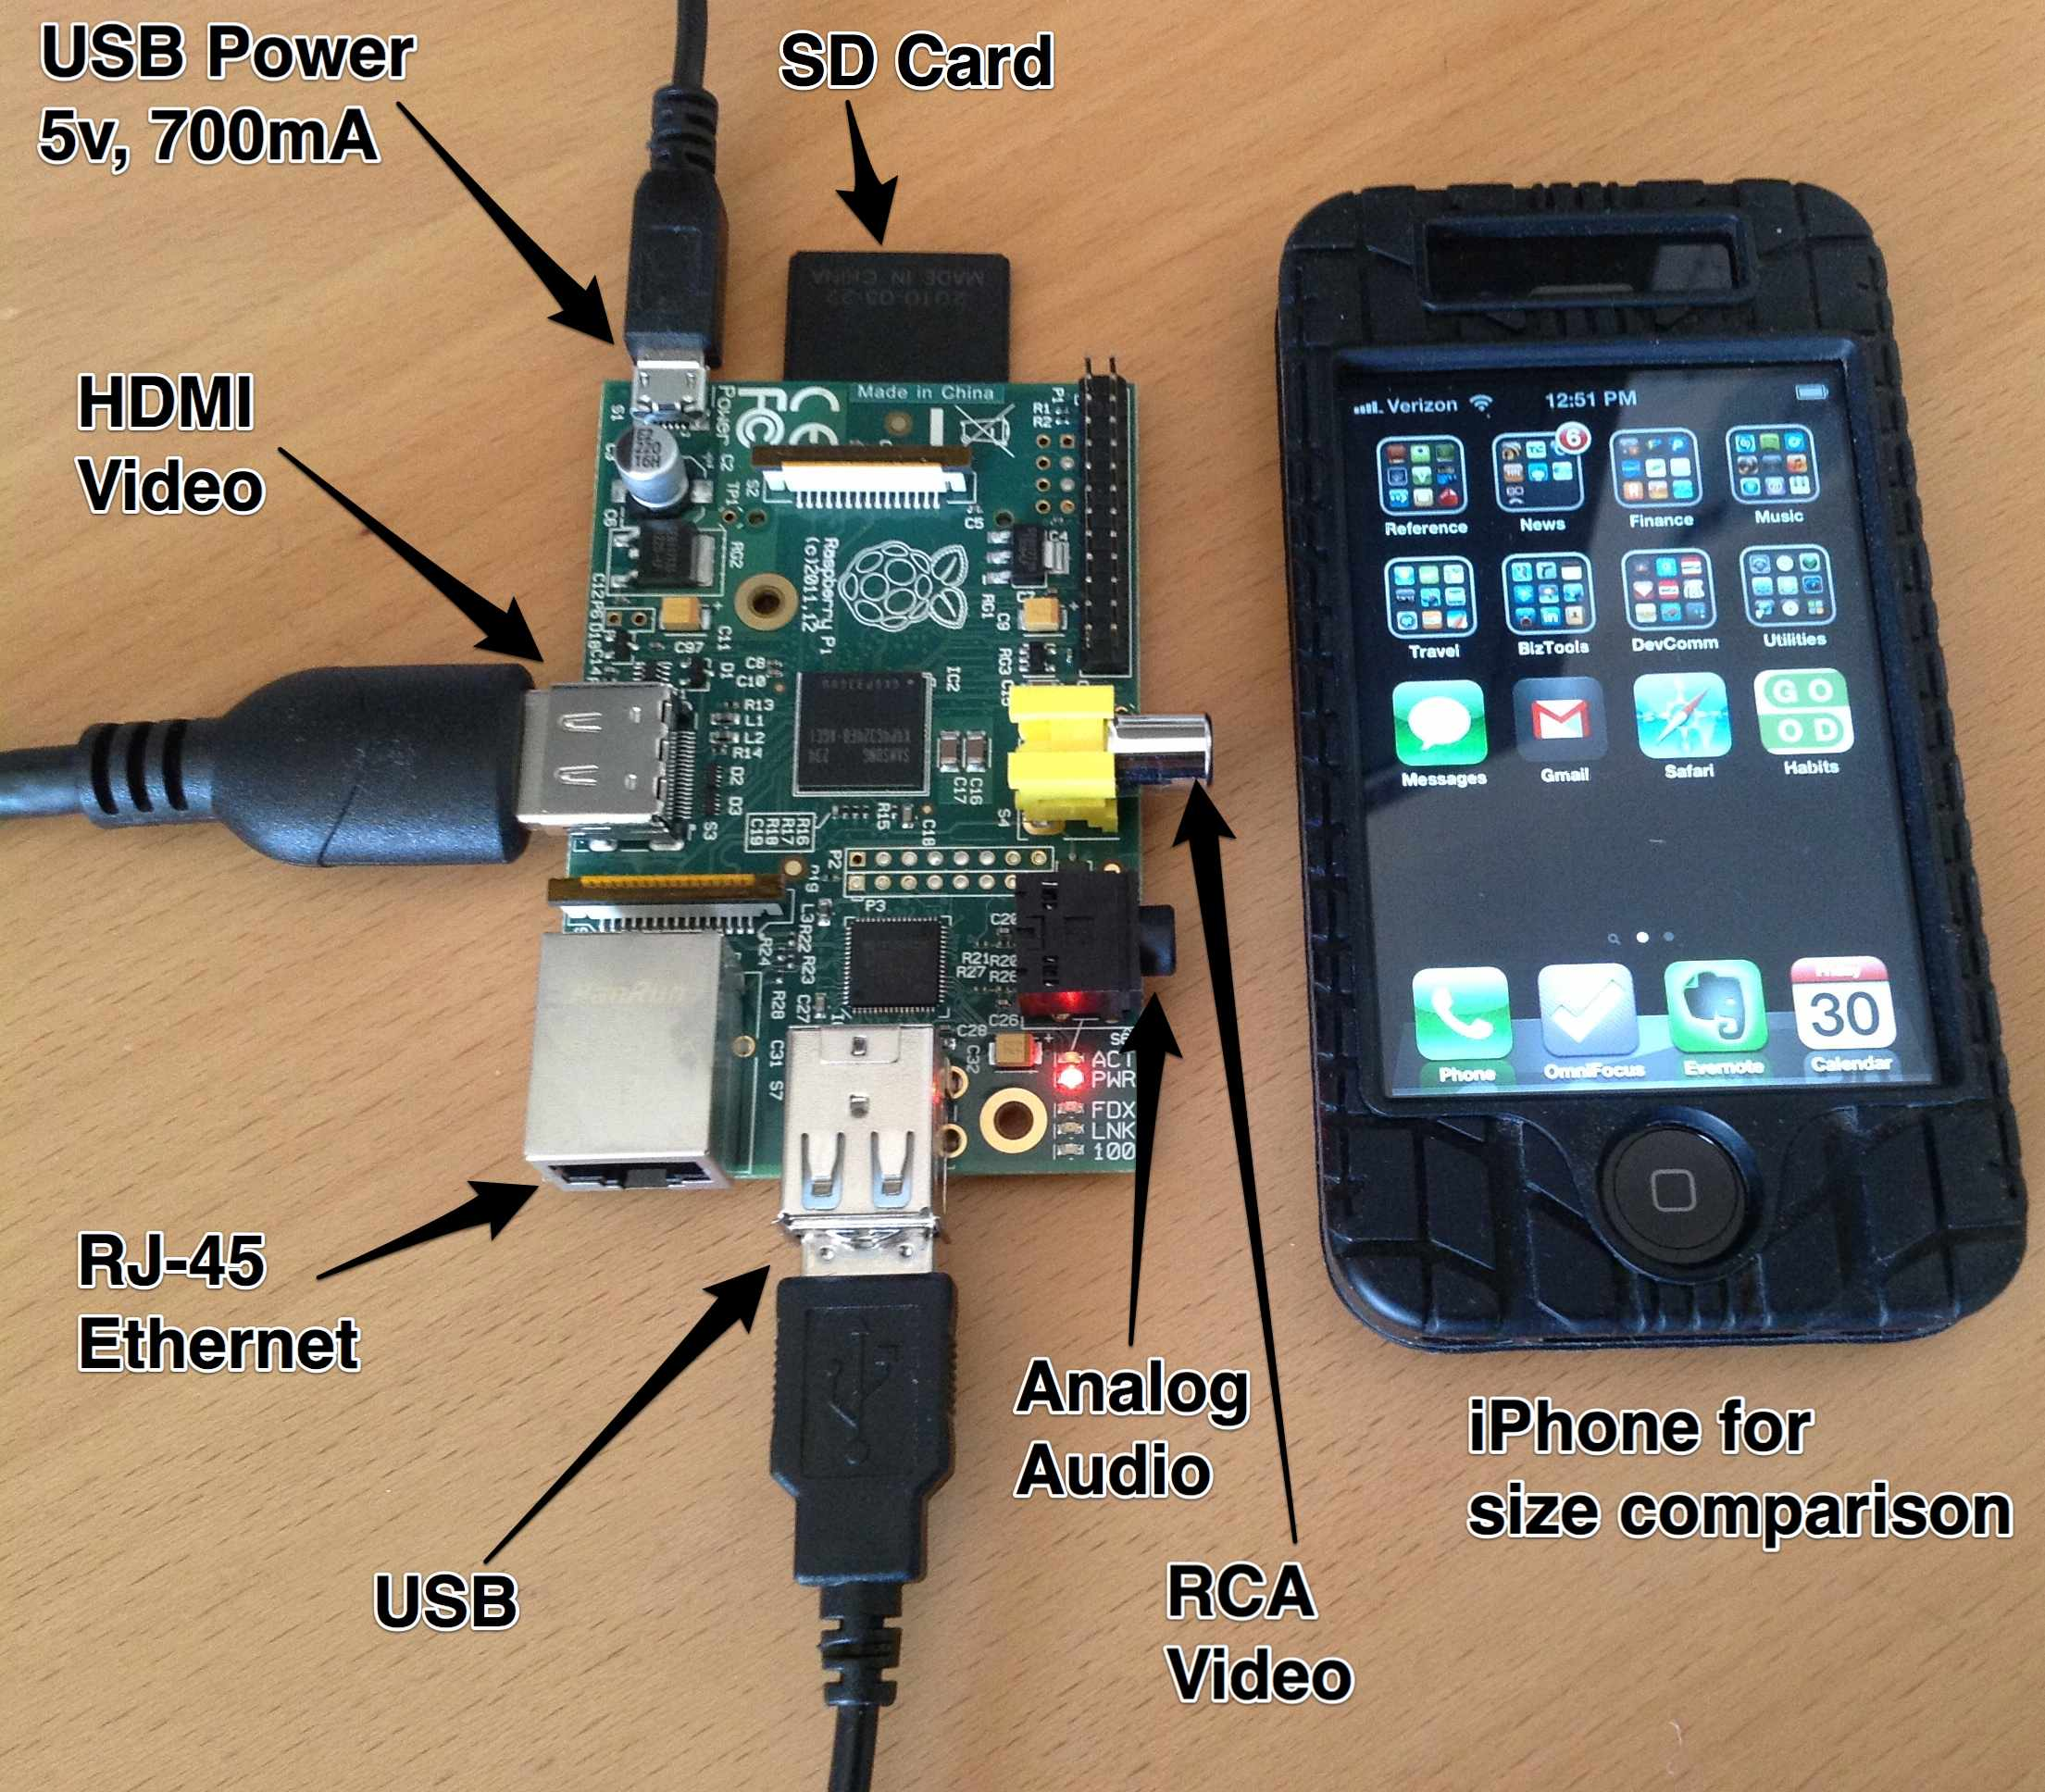
\includegraphics[scale=0.1]{imagenes/raspberry_pi_iphone.jpg}
\caption{Tarjeta Raspberry Pi con descripción de los puertos}
\end{figure}

\begin{itemize}
\item Camara Raspberry Pi: Es un sensor encargado de captar imagenes y grabar videos de alta definicion. Se conecta a la
Raspberry Pi con un cable de cinta plana de 15 cm en el puerto CSI. Tiene 5 megapíxeles de foco fijo que soporta los modos
de vídeo de 1080x30, 720x60 y VGA90. Puede ser manejada con las librerías MMAL, V4L u otras librerías de terceros como la de
Python. \cite{raspberrycam} %(http://www.raspberrypi.org/products/camera-module/)

\end{itemize}

\begin{figure}[hbtp]
\centering
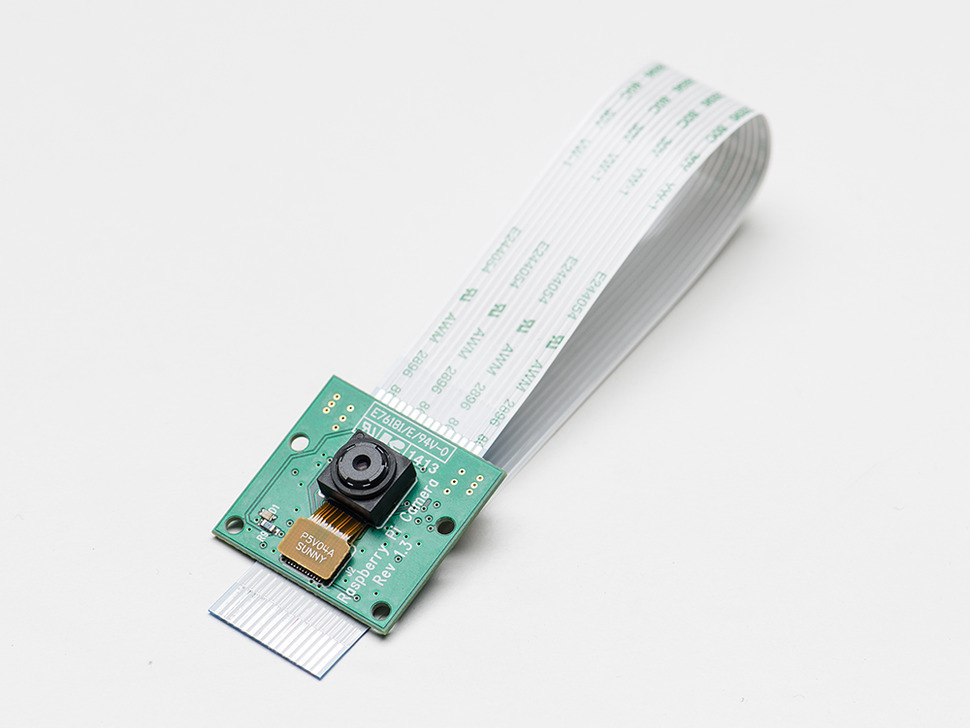
\includegraphics[scale=0.7]{imagenes/1367-01.jpg}
\caption{Camara Raspberry Pi}
\end{figure}


\begin{itemize}
\item Batería de polímero de litio (Lipo): Es la fuente de poder usada para que los motores y componentes electronicos
funcionen. La batería usada es de 11.1 voltios y 1 amperio. \cite{bateria}
\end{itemize}


\begin{figure}[hbtp]
\centering
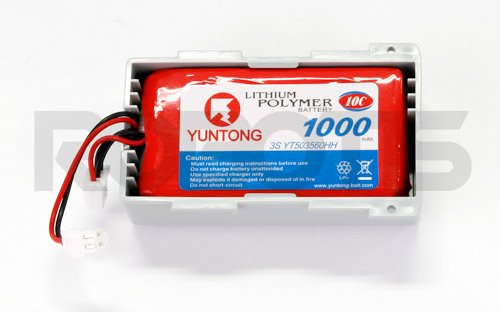
\includegraphics[scale=0.5]{imagenes/R-LIPOBAT.jpg}
\caption{Batería Lipo}
\end{figure}

\begin{itemize}
\item Circuito con regulador de 5v: Es un circuito diseñado y construido para este proyecto cuya finalidad es regular la 
entrada de la corriente. Por una de las salidas se expulsa 5v y por la otra se mantiene el mismo voltaje de entrada. 
\end{itemize}

%\begin{figure}[hbtp]
%\centering
%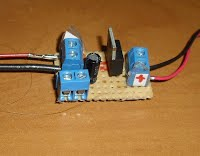
\includegraphics[scale=0.7]{imagenes/circuito.jpg}
%\caption{Lipo}
%\end{figure}



